\documentclass[tikz,border=7pt]{standalone}
\usepackage[T1]{fontenc}
\usepackage{lmodern}
\usetikzlibrary{arrows.meta,positioning,shapes.geometric,fit,backgrounds,calc}
\begin{document}
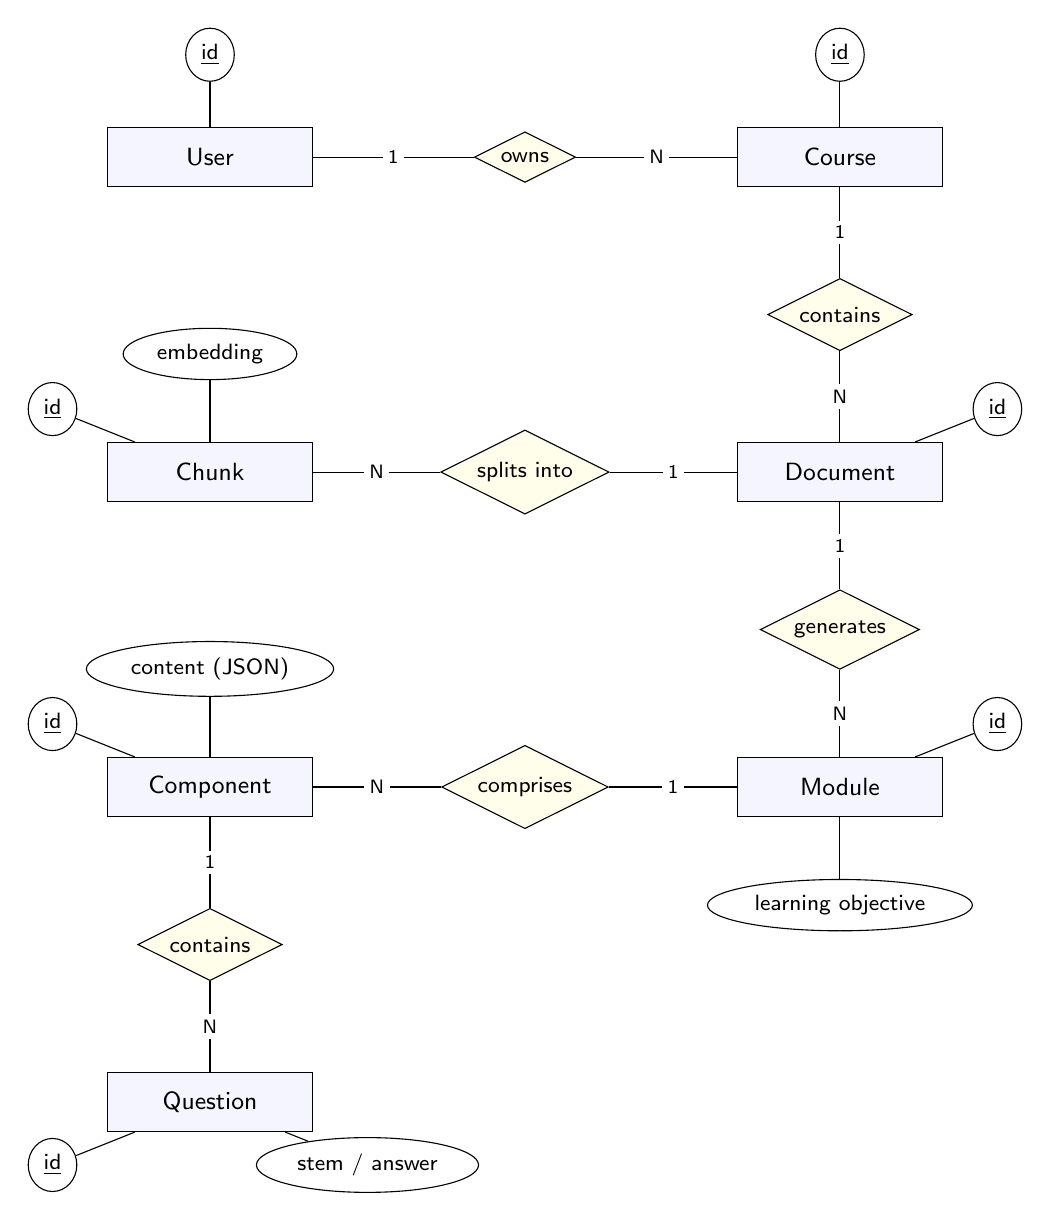
\begin{tikzpicture}[font=\sffamily\small,>=Latex,
box/.style={draw,rounded corners=2pt,align=center,minimum width=3cm,minimum height=1cm,fill=blue!4},
entity/.style={draw,rectangle,align=center,minimum width=2.6cm,minimum height=.75cm,fill=blue!4},
rel/.style={draw,diamond,aspect=2,inner sep=2pt,align=center,font=\sffamily\footnotesize,fill=yellow!8},
attr/.style={draw,ellipse,inner sep=3pt,font=\sffamily\footnotesize},
uc/.style={draw,ellipse,align=center,minimum width=4cm,minimum height=.9cm},
flow/.style={->,thick},lab/.style={font=\sffamily\scriptsize,fill=white,inner sep=2pt}]
\node[entity] (u) at (0,9) {User};
\node[entity] (c) at (8,9) {Course};
\node[entity] (d) at (8,5) {Document};
\node[entity] (ch) at (0,5) {Chunk};
\node[entity] (m) at (8,1) {Module};
\node[entity] (co) at (0,1) {Component};
\node[entity] (q) at (0,-3) {Question};
\node[rel] (owns) at (4,9) {owns}; \draw (u) -- node[lab]{1} (owns); \draw (owns) -- node[lab]{N} (c);
\node[rel] (hasdoc) at (8,7) {contains}; \draw (c) -- node[lab]{1} (hasdoc); \draw (hasdoc) -- node[lab]{N} (d);
\node[rel] (chunks) at (4,5) {splits into}; \draw (d) -- node[lab]{1} (chunks); \draw (chunks) -- node[lab]{N} (ch);
\node[rel] (source) at (8,3) {generates}; \draw (d) -- node[lab]{1} (source); \draw (source) -- node[lab]{N} (m);
\node[rel] (comps) at (4,1) {comprises}; \draw (m) -- node[lab]{1} (comps); \draw (comps) -- node[lab]{N} (co);
\node[rel] (questions) at (0,-1) {contains}; \draw (co) -- node[lab]{1} (questions); \draw (questions) -- node[lab]{N} (q);
\node[attr] (uid) at (0,10.3) {\underline{id}}; \draw (u) -- (uid);
\node[attr] (cid) at (8,10.3) {\underline{id}}; \draw (c) -- (cid);
\node[attr] (did) at (10,5.8) {\underline{id}}; \draw (d) -- (did);
\node[attr] (chid) at (-2,5.8) {\underline{id}}; \draw (ch) -- (chid);
\node[attr] (vec) at (0,6.5) {embedding}; \draw (ch) -- (vec);
\node[attr] (mid) at (10,1.8) {\underline{id}}; \draw (m) -- (mid);
\node[attr] (lo) at (8,-0.5) {learning objective}; \draw (m) -- (lo);
\node[attr] (coid) at (-2,1.8) {\underline{id}}; \draw (co) -- (coid);
\node[attr] (json) at (0,2.5) {content (JSON)}; \draw (co) -- (json);
\node[attr] (qid) at (-2,-3.8) {\underline{id}}; \draw (q) -- (qid);
\node[attr] (stem) at (2,-3.8) {stem / answer}; \draw (q) -- (stem);
\end{tikzpicture}
\end{document}
